\section{Auswertung}
\label{sec:Auswertung}
Sämtliche im Folgenden durchgeführten Ausgleichsrechnungen werden mit der \emph{curve fit} Funktion aus dem für \emph{Python} geschriebenen package \emph{NumPy}\cite{scipy} durchgeführt. Fehlerrechnungen werden mit dem für \emph{Python} geschriebenen package \emph{Uncertainties}\cite{uncertainties} ausgeführt.

\subsection{Allgemeine Auswertung der Filmstreifen}
\label{sec:allgemein}
Zur Auswertung wird der Nullpunkt in die Mitte des linken ausgestanzten Loches gesetzt, da in diesem Punkt der Strahl die Kamera verlässt. Somit entspricht der Abstand zwischen beiden ausgestanzten Löchern einem Winkel von $\theta=\pi$. Der Abstand der Streifen zum Nullpunkt werden mit einem Geodreik vermessen und mit der Beziehung
\begin{align}
	\theta=\frac{s}{2R}
\end{align}
in den Beugungswinkel überführt. Dabei beschreibt $s$ den Abstand des auftretenen Reflex zum Nullpunkt und $R$ den Radius der verwendeten Kamera.  Aufgrund der Fehleranfälligkeit die beim ablesen besteht, wird auf jeden Reflex ein Unsicherheit von einem Millimeter angenommen.
Der Netzebenabstand $d$ wird darauf hin, unter Verwendung der Bragg-Bedingung XXX, bestimmt.
\subsection{Metallprobe}
Die im voherigen Kapitel beschriebenen Messgrößen sind in Tabelle
% \ref{table:A1}
für die verwendete Metallprobe 9 zusammengefasst.
\begin{table}
    \centering
    \caption{Messdaten der Metallprobe.}
    \label{table:A1}
    \sisetup{parse-numbers=false}
    \begin{tabular}{
	S[table-format=2.1]
	@{${}\pm{}$}
	S[table-format=1.1, table-number-alignment = left]
	S[table-format=1.3]
	@{${}\pm{}$}
	S[table-format=1.3, table-number-alignment = left]
	S[table-format=1.3]
	@{${}\pm{}$}
	S[table-format=1.3, table-number-alignment = left]
	}
	\toprule
	\multicolumn{2}{c}{$s\:/\: \si{\centi\meter}$}		& \multicolumn{2}{c}{$\theta\:/\: \si{\centi\meter}$}		&
    \multicolumn{2}{c}{$d \:/\: \si{\angstrom}$}		\\ 
	\midrule
    4.0  & 0.1 & 0.349 & 0.009 & 2.25   & 0.05   \\
5.7  & 0.1 & 0.497 & 0.009 & 1.62   & 0.03   \\
7.1  & 0.1 & 0.620 & 0.009 & 1.33   & 0.02   \\
8.4  & 0.1 & 0.733 & 0.009 & 1.15   & 0.01   \\
9.6  & 0.1 & 0.838 & 0.009 & 1.037  & 0.008  \\
10.9 & 0.1 & 0.951 & 0.009 & 0.947  & 0.006  \\
12.2 & 0.1 & 1.065 & 0.009 & 0.881  & 0.004  \\
13.8 & 0.1 & 1.204 & 0.009 & 0.826  & 0.003  \\
16.2 & 0.1 & 1.414 & 0.009 & 0.780  & 0.001  \\
16.4 & 0.1 & 1.435 & 0.009 & 0.7795 & 0.0009 \\

    \bottomrule
    \end{tabular}
    \end{table}

Zur Bestimmung der Kristallstruktur wird das Verhältnis
\begin{align}
	\frac{d_1}{d_i}=\frac{m_i}{m_1}
	\label{eq:dm}
\end{align}
verwendet, wobei gilt $m=\sqrt{h^2+k^2+l^2}$.
In Tabelle
%\ref{table:A2}
sind die ersten neun Reflexe der Kristallstrukturen
simple-cubic (sc),body centered cubic (bbc), face centered cubic (fcc)
und Diamant aufgelistet, zudem wird das in Gleichung
%$\ref{eq:dm}
 beschriebene Verhältnis gebildet, um diese mit der Probe zu vergleichen.


\begin{table}
    \centering
    \caption{Vergleich der Verhältnisse für die Metallprobe.}
    \label{table:A2}
    \sisetup{parse-numbers=false}
    \begin{tabular}{
	S[table-format=3.0]
	S[table-format=1.2]
	S[table-format=3.0]
	S[table-format=1.2]
	S[table-format=3.0]
	S[table-format=1.2]
	S[table-format=3.0]
	S[table-format=1.2]
	S[table-format=1.2]
	@{${}\pm{}$}
	S[table-format=1.2, table-number-alignment = left]
	}
	\toprule
	{$\text{sc}$}		& {$\left(\frac{m_i}{m_1}\right)_{sc}$}		& 
	{$\text{bcc}$}		& {$\left(\frac{m_i}{m_1}\right)_{bcc}$}		& 
	{$\text{fcc}$}		& {$\left(\frac{m_i}{m_1}\right)_{fcc}$}		& 
	{$\text{diamant}$}		& {$\left(\frac{m_i}{m_1}\right)_{dia}$}		& 
	\multicolumn{2}{c}{$\frac{d_1}{d_i}$}		\\ 
	\midrule
    100 & 1.00 & 110 & 1.00 & 111 & 1.00 & 111 & 1.00 & 1.0  & 0    \\
110 & 1.41 & 200 & 1.41 & 200 & 1.15 & 220 & 1.63 & 1.40 & 0.04 \\
111 & 1.73 & 211 & 1.73 & 220 & 1.63 & 311 & 1.91 & 1.70 & 0.05 \\
200 & 2.00 & 220 & 2.00 & 311 & 1.91 & 400 & 2.31 & 1.96 & 0.05 \\
210 & 2.24 & 310 & 2.24 & 222 & 2.00 & 331 & 2.52 & 2.17 & 0.05 \\
211 & 2.45 & 222 & 2.45 & 400 & 2.31 & 422 & 2.83 & 2.38 & 0.06 \\
220 & 2.83 & 321 & 2.65 & 331 & 2.52 & 333 & 3.00 & 2.56 & 0.06 \\
221 & 3.00 & 400 & 2.83 & 420 & 2.58 & 440 & 3.27 & 2.73 & 0.07 \\
310 & 3.16 & 330 & 3.00 & 422 & 2.83 & 531 & 3.42 & 2.90 & 0.07 \\

    \bottomrule
    \end{tabular}
    \end{table}


Der Vergleich mit allen Strukturen zeigt, dass die Probe eine bcc-Struktur besitzt.
Desweiteren ist die Gitterkonstante $a$ der Probe zu bestimmen. Diese wird nach Gleichung XXX berechnet und in Abbildung \ref{fig:plot1} gegen $\cos^2{(\theta)}$ aufgetragen. Durch die verwendete lineare Ausgleichsrechnung
\begin{align}
	a(\cos{(\theta)})= b\cos^2{(\theta)} + c
\end{align}

\begin{figure}
  \centering
  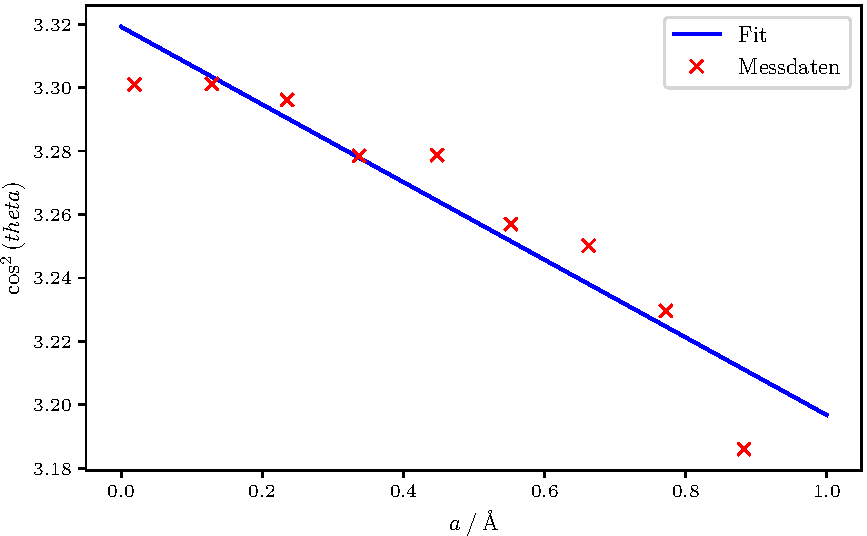
\includegraphics{build/Metall.pdf}
  \caption{Messdaten und Fitergebnis.}
  \label{fig:plot1}
\end{figure}

werden die in Kapitel XXX angesprochenen systematischen Fehler korrigiert. Die resultierenden Fitparamter lauten:
\begin{align}
	b&= \SI{-0.125+-0.016}{\angstrom}
 \\
	c&= \SI{3.3192+-0.0087}{\angstrom}

\end{align}

Die Gitterkonstante und die vorliegende bcc-Struktur weißt nach \cite{gitter} auf Niob hin. Die Abweichung zur der in der Literatur angegebenen Gitterkonstante
$a=\SI{3.30}{\angstrom}$ beträgt $\SI{1.038+-0.005}{\percent}
$.





% % Examples
% \begin{equation}
%   U(t) = a \sin(b t + c) + d
% \end{equation}
%
% \begin{align}
%   a &= \input{build/a.tex} \\
%   b &= \input{build/b.tex} \\
%   c &= \input{build/c.tex} \\
%   d &= \input{build/d.tex} .
% \end{align}
% Die Messdaten und das Ergebnis des Fits sind in Abbildung~\ref{fig:plot} geplottet.
%
% %Tabelle mit Messdaten
% \begin{table}
%   \centering
%   \caption{Messdaten.}
%   \label{tab:data}
%   \sisetup{parse-numbers=false}
%   \begin{tabular}{
% % format 1.3 bedeutet eine Stelle vorm Komma, 3 danach
%     S[table-format=1.3]
%     S[table-format=-1.2]
%     @{${}\pm{}$}
%     S[table-format=1.2]
%     @{\hspace*{3em}\hspace*{\tabcolsep}}
%     S[table-format=1.3]
%     S[table-format=-1.2]
%     @{${}\pm{}$}
%     S[table-format=1.2]
%   }
%     \toprule
%     {$t \:/\: \si{\milli\second}$} & \multicolumn{2}{c}{$U \:/\: \si{\kilo\volt}$\hspace*{3em}} &
%     {$t \:/\: \si{\milli\second}$} & \multicolumn{2}{c}{$U \:/\: \si{\kilo\volt}$} \\
%     \midrule
%     \input{build/table.tex}
%     \bottomrule
%   \end{tabular}
% \end{table}
%
% % Standard Plot
% \begin{figure}
%   \centering
%   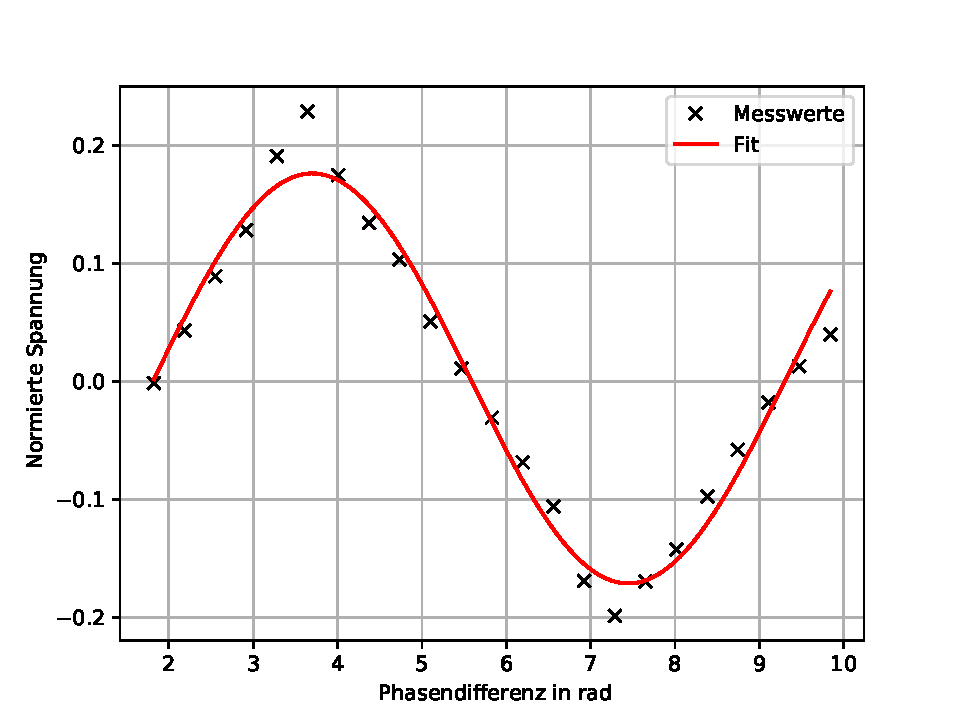
\includegraphics{build/plot.pdf}
%   \caption{Messdaten und Fitergebnis.}
%   \label{fig:plot}
% \end{figure}
%
% 2x2 Plot
% \begin{figure*}
%     \centering
%     \begin{subfigure}[b]{0.475\textwidth}
%         \centering
%         \includegraphics[width=\textwidth]{Abbildungen/Schaltung1.pdf}
%         \caption[]%
%         {{\small Schaltung 1.}}
%         \label{fig:Schaltung1}
%     \end{subfigure}
%     \hfill
%     \begin{subfigure}[b]{0.475\textwidth}
%         \centering
%         \includegraphics[width=\textwidth]{Abbildungen/Schaltung2.pdf}
%         \caption[]%
%         {{\small Schaltung 2.}}
%         \label{fig:Schaltung2}
%     \end{subfigure}
%     \vskip\baselineskip
%     \begin{subfigure}[b]{0.475\textwidth}
%         \centering
%         \includegraphics[width=\textwidth]{Abbildungen/Schaltung4.pdf}    % Zahlen vertauscht ... -.-
%         \caption[]%
%         {{\small Schaltung 3.}}
%         \label{fig:Schaltung3}
%     \end{subfigure}
%     \quad
%     \begin{subfigure}[b]{0.475\textwidth}
%         \centering
%         \includegraphics[width=\textwidth]{Abbildungen/Schaltung3.pdf}
%         \caption[]%
%         {{\small Schaltung 4.}}
%         \label{fig:Schaltung4}
%     \end{subfigure}
%     \caption[]
%     {Ersatzschaltbilder der verschiedenen Teilaufgaben.}
%     \label{fig:Schaltungen}
% \end{figure*}
